Loci can be elliptic, non-elliptic, or even a point. But can they be circular? And to boot, stationary?

Let $P$ be an orbit's vertex and $P'$ its reflection about the origin, also on $B$, 
Figure~\ref{fig:cosine_circle_construction}. Let  $Q_1$ and $Q_2$ be intersections of the tangent to $B$ at $P'$ with the orbit's Excentral Triangle $T'$. The following remarkable property is verified, illustrated in Figure~\ref{fig:cosine_circle_locus}: 


\begin{theorem}
The locus of $Q_1$ (or $Q_2$) is a {\em stationary circle}, and its center is the billiard's.
\end{theorem}

\begin{figure}[H]
     \centering
     \begin{subfigure}[t]{0.45\textwidth}
         \centering
         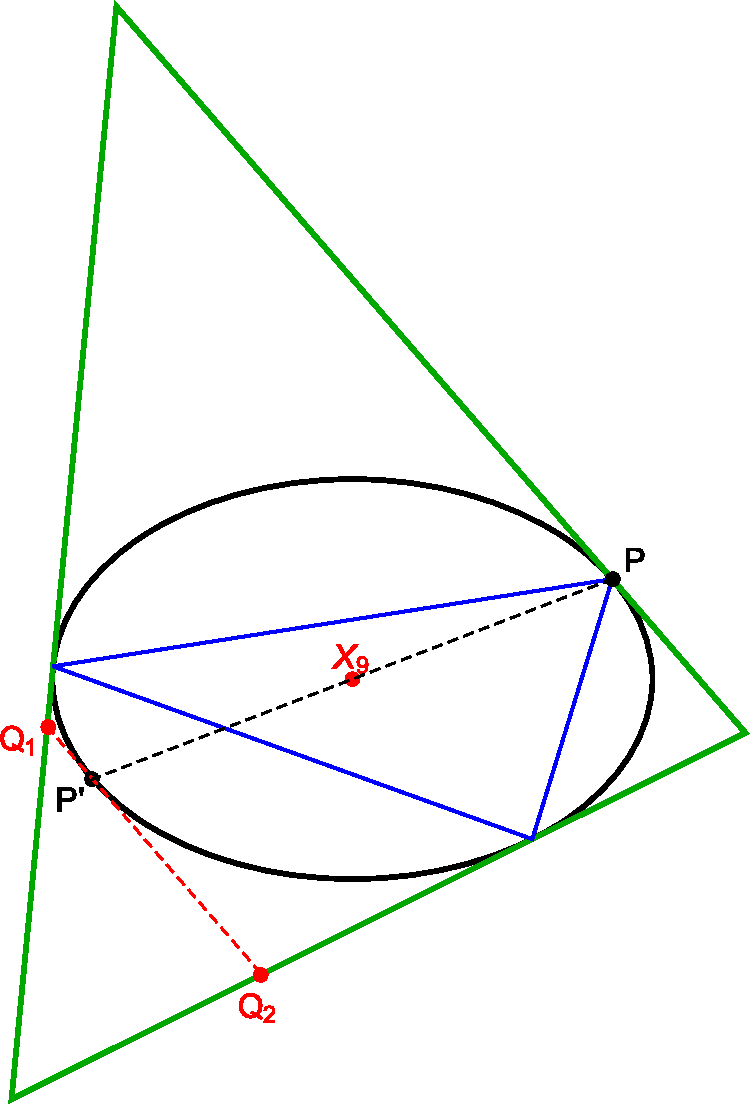
\includegraphics[width=1.0\linewidth]{pics/0100_cosine_circle_construction.pdf}
    \caption{Stationary Circle Construction.}
    \label{fig:cosine_circle_construction}
     \end{subfigure}
     \hfill
     \begin{subfigure}[t]{0.45\textwidth}
         \centering
          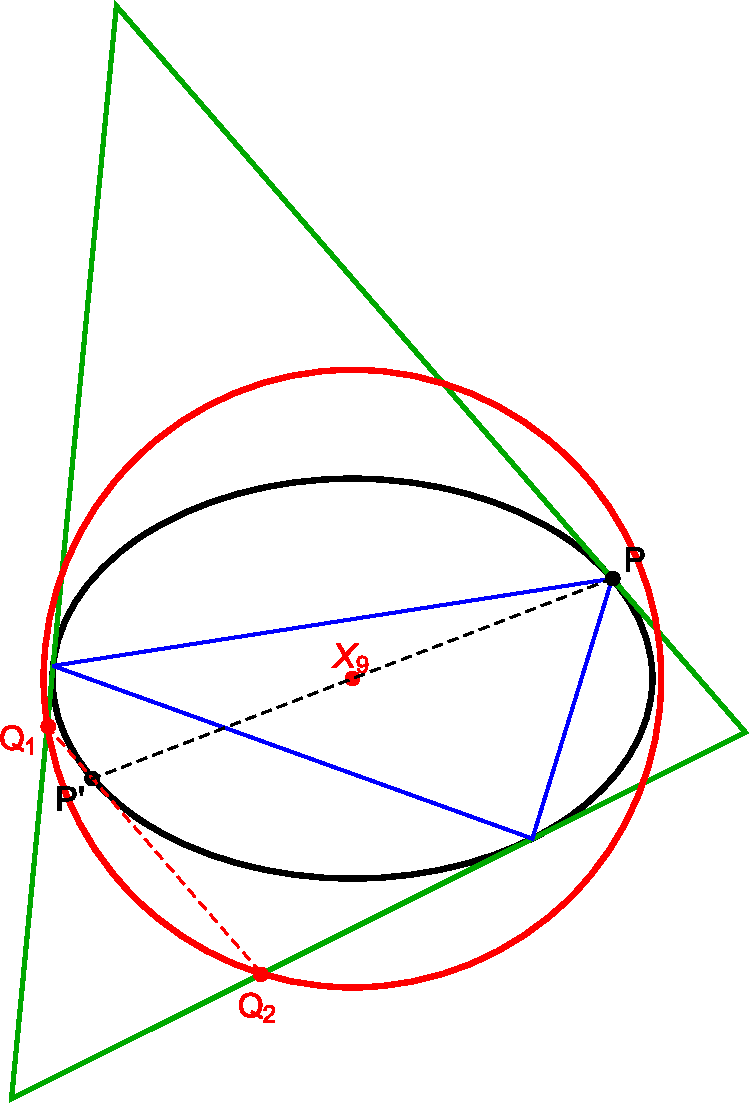
\includegraphics[width=1.0\linewidth]{pics/0110_cosine_circle_locus.pdf}
         \caption{Circular Locus of $Q_1$ (or $Q_2$).}
         \label{fig:cosine_circle_locus}
     \end{subfigure}
     \caption{Construction of Circular Locus.}
\end{figure}

The radius $r^*$ of this circle is given by \cite{ronaldo19a}:

\begin{equation}
r^* = \frac{\sqrt{3}}{3}\sqrt{2\delta+a^2+1}\,>\,a
\label{eqn:rstar}
\end{equation}

It turns out, the above locus is congruent with the {\em Cosine Circle} of the Excentral Triangle, also known as its {\em Second Lemoine Circle} \cite{mw}. Its center is known to lie on the Symmedian Pointof the Excentral, known to be congruent with the Mittenpunkt $X_9$, stationary in our case. The radius of the Cosine Circle can also be stated as a function of the constant perimeter $L$ and momentum $\gamma$ \cite{dominique19,sergei19_private_circles}:

\begin{equation}
    r^* = \frac{L}{\frac{r}{R}+4} = \frac{1}{\gamma}
\end{equation}

Also notable is the Excentral's {\em Cosine Hexagon} \cite{mw} whose six vertices are concyclic with the Cosine Circle \cite{mw}. Remarkably, its six sides will be either parallel to the orbit's or tangent to the billiard, Figure~\ref{fig:cosine_hexagon}. The vertices for the Excentral Cosine Hexagon can also be constructed by intersecting the orbit's Excentral Triangle with its copy reflected about the Billiard center, \ref{fig:cosine_circle_excentral_hexagon}

No other {\em Tucker Circles} \cite{mw} for the $N=3$ family have been found to be stationary.

\begin{figure}[H]
     \centering
     \begin{subfigure}[t]{0.45\textwidth}
         \centering
          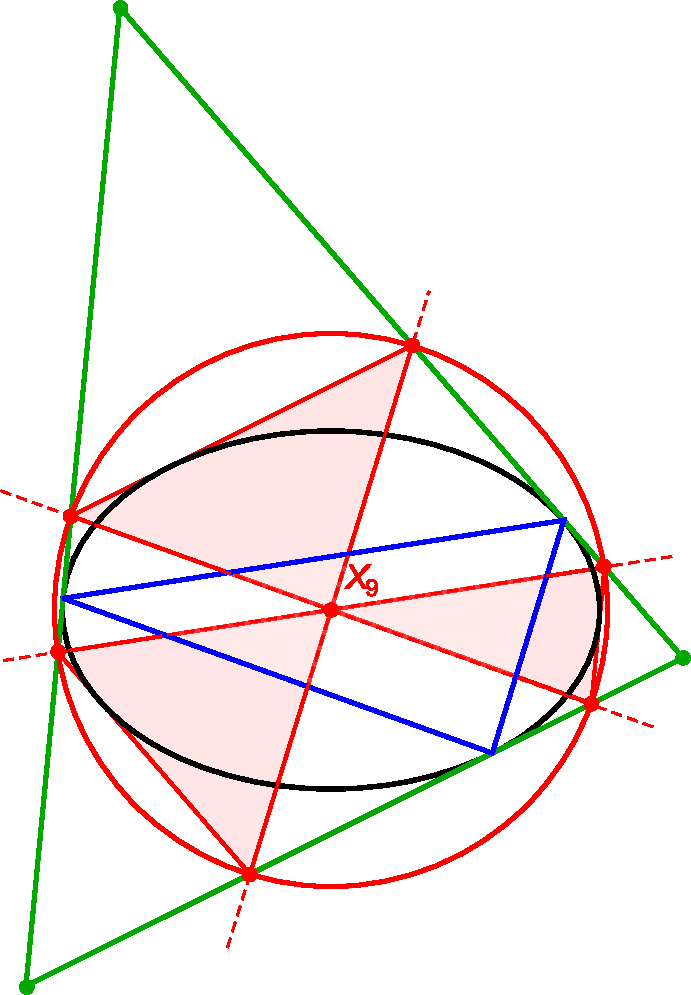
\includegraphics[width=1.0\linewidth]{pics/0130_cosine_hexagon.pdf}
         \caption{The vertices of the Excentral's Cosine Hexagon are the intersections of antiparallels (lines parallel to the Orthic, which in our case is the orbit) drawn through the Symmedian of the Excentral (congruent with the Mittenpunkt of the orbit and therefore stationary). These vertices are concyclic on the stationary Cosine Circle.}
     \label{fig:cosine_hexagon}
     \end{subfigure}
    \hfill
     \begin{subfigure}[t]{0.45\textwidth}
         \centering
         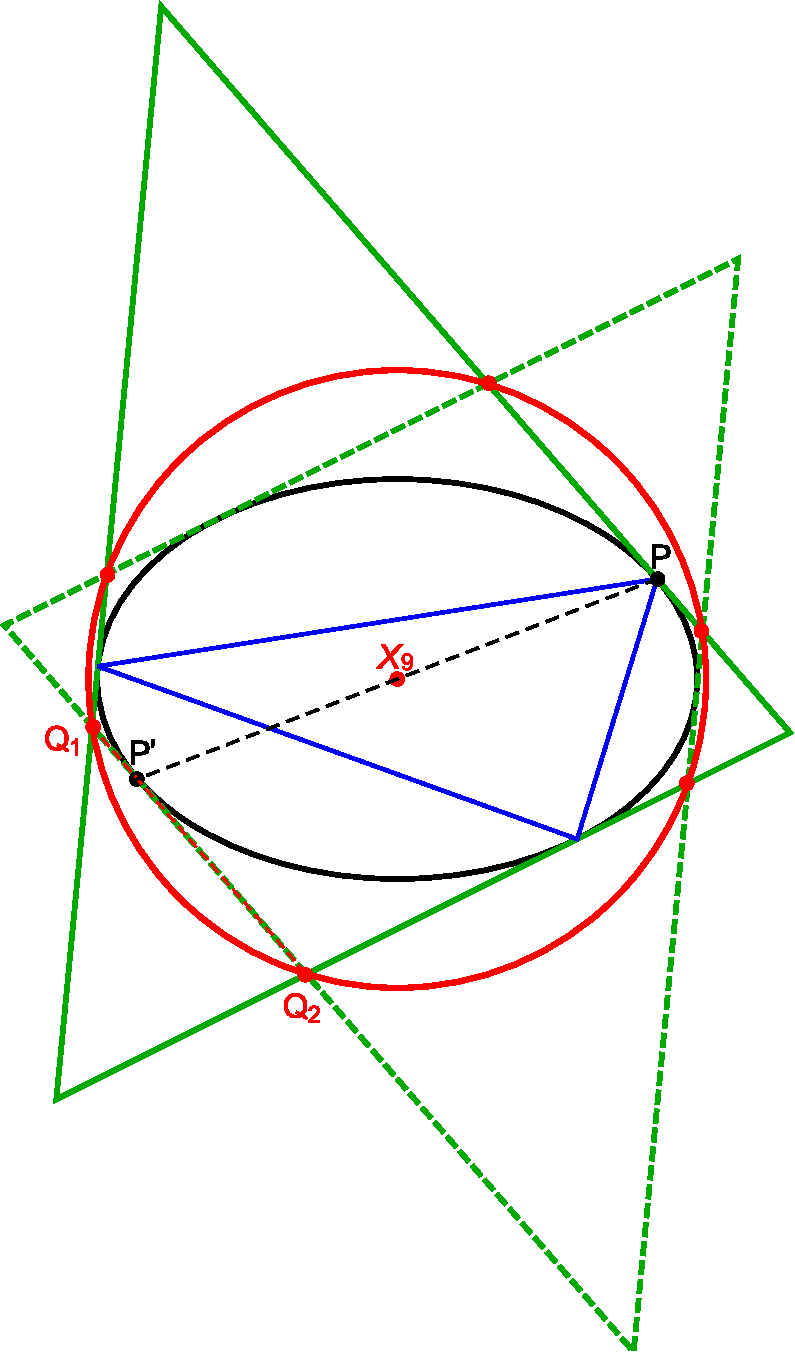
\includegraphics[width=1.0\linewidth]{pics/0120_cosine_circle_reflected_excentral.pdf}
    \caption{The Excentral Triangle intersects its reflection about the Symmedian on the six vertices of its Cosine Hexagon. Their locus is the Excentral's stationary Cosine Circle.}
    \label{fig:cosine_circle_excentral_hexagon}
     \end{subfigure}
     \caption{Two constructions for the concyclic vertices of the Excentral's Cosine Hexagon, whose locus is a stationary circle.}
\end{figure}

A video of this surprising phenomenon is available here \cite[video \#8]{dsr_main_videos_2019}.
